\chapter{Result Analysis}
\label{ch04}
The analysis of the work results is provided in this chapter. As described in Section \ref{ch03:analysis}, the analysis is divided into two topics: \textit{(i)} evolution of catchment areas (Section \ref{ch04:evolution}), and \textit{(ii)} the differences between IPv4 and IPv6 catchment areas (Section \ref{ch04:differences}). The features of visualization tool intended to help operator assessing their catchment areas is discussed in Section \ref{ch04:visualizing}. Finally, this chapter is concluded by a discussion about the importance of performing IPv4/IPv6 catchment areas for the operator in Section \ref{ch04:discussion}.

\section{Evolution of Catchment Areas}
\label{ch04:evolution}
Over the time, anycast operators may made changes on their network in order to improve the service. They may have added instances at underserved locations, changed their service policy, made new peering agreements with other organizations, and so on. These changes may result in congruity of the IPv4 and IPv6 catchments, or even higher differences between them. The changes may also not fundamental enough to change the catchment topology, hence it remains relatively the same throughout time. In this subsection, we discuss about the evolution of Root Server's catchment areas from control-plane perspective during the period March 1\textsuperscript{st} 2008 to June 1\textsuperscript{st} 2016.

\subsection{Convergence}
\label{ch04:evolution:convergence}
Recalling from Section \ref{ch03:analysis:evolution}, convergence level is a metric to describe the fraction of converging VPs of all dual-stacked VPs that see certain Root Server prefixes. Convergence levels of all Root Servers are presented in Appendix \ref{app:convergence}, with some are presented in Figure \ref{fig:ch04:convergence}. The blue line represents the convergence level, and the red line indicates the total number of dual-stacked VPs. The inclusion of the dual-stacked VPs into the graphs serves two purposes: \textit{(i)} it can be used as the control when there is outlier data for convergence level. For example, K-Root (Figure \ref{fig:convergence-k}) have convergence level 100\% until the middle of 2009. By observing the number of VPs at the same time period, it is because there was only small number of VPs detected K-Root prefixes hence the skewed result. \textit{(ii)} it can also be used to infer the visibility level of Root Servers as seen by RIS peers, as explained later in this subsection. 

The results show that convergence level of the majority of the Root Servers is relatively high, between 50\% to 80\%, with the exception J- and M-Root that are below 40\%. Most Root Servers’ convergence are varying over the time, which implies that network changes took place during the period. In general, they have tendency to increase over the time. Some experience sharp increase at one point in time (A, D), some are steadily increasing (K, L), and some are relatively stagnated (I, C). Only D and M-Root that experience a notable temporary decreasing moment.

\begin{figure}[h]
	\begin{subfigure}{.5\textwidth}
		\centering
		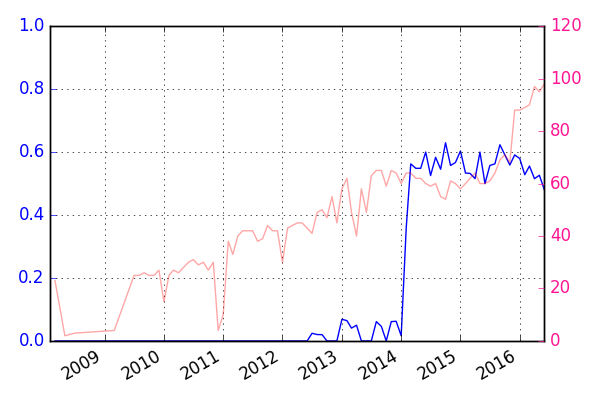
\includegraphics[width=.8\linewidth]{img/convergence_over_time_a}
		\caption{A-Root}
		\label{fig:ch04:convergence_a}
	\end{subfigure}
	\begin{subfigure}{.5\textwidth}
		\centering
		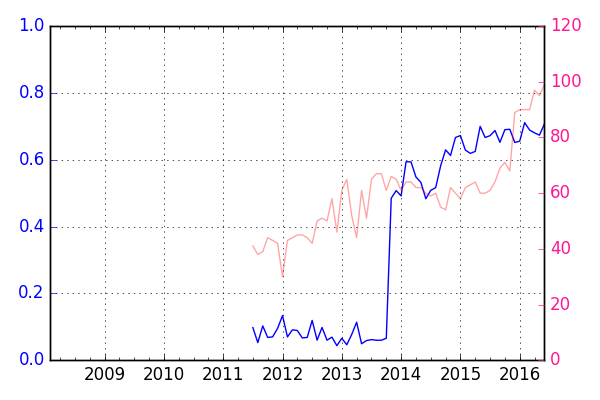
\includegraphics[width=.8\linewidth]{img/convergence_over_time_d}
		\caption{D-Root}
		\label{fig:ch04:convergence_d}
	\end{subfigure}
	\begin{subfigure}{.5\textwidth}
		\centering
		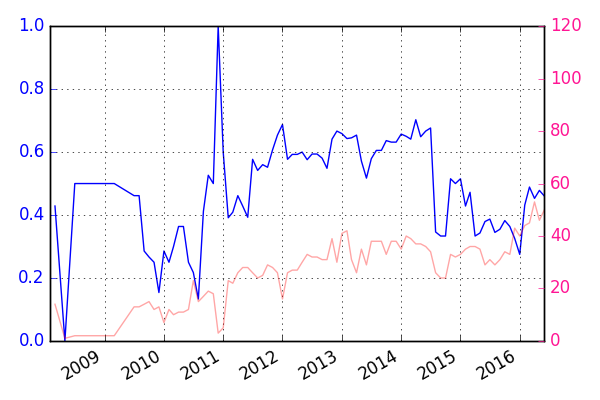
\includegraphics[width=.8\linewidth]{img/convergence_over_time_f}
		\caption{F-Root}
		\label{fig:ch04:convergence_f}
	\end{subfigure}
	\begin{subfigure}{.5\textwidth}
		\centering
		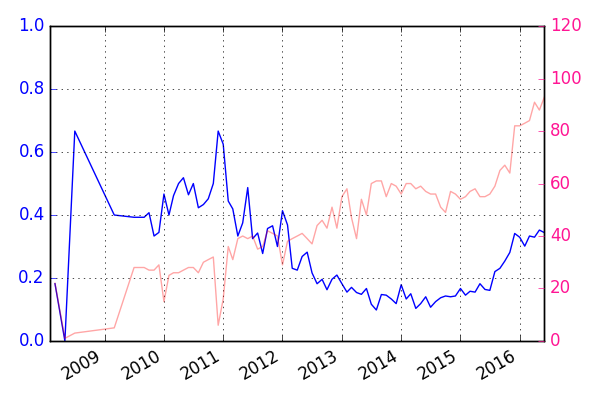
\includegraphics[width=.8\linewidth]{img/convergence_over_time_m}
		\caption{M-Root}
		\label{fig:ch04:convergence_m}
	\end{subfigure}	
	\caption{Convergence level of A, F, D, and M-Root. Results for others are available in Appendix \ref{app:convergence}}
	\label{fig:ch04:convergence}
\end{figure}

From the convergence graphs, a number of notable events can be noticed. Obviously, not all events can be explained since it requires the knowledge of complete routing policies implemented at the routers, which is not available in our datasets. Nevertheless, using the BGP routing data obtained from RIPEStat, some events can be explored as the following. 

\subsubsection{Dramatic Increase of A- and D-Root}
The common feature from A- (Figure \ref{fig:ch04:convergence_a}) and D-Root (Figure \ref{fig:ch04:convergence_d}) is that they experience dramatic increase at some point in time. 

A-Root is identified to have significant increase in February 2014. To analyze this, we compare data on January 1\textsuperscript{st} 2014 and February 1\textsuperscript{st} 2014. There are 60 and 64 dual-stacked VPs respectively, without any VP from January was absent in the subsequent month. Initially there was only one converging VP, then the number increased to 18 in February. 14 out of those 18 VPs converged due to the change in origin AS for IPv6 prefix (from AS 36623 to AS 36625). Recall from Section \ref{ch02:measuring-anycast} that A-Root originate their prefixes from multiple ASes, possibly one AS per instance\footnote{unfortunately, we cannot find official information available for confirmation}. One major factor contributing in low convergence level of A-Root is due to the difference of IPv4/IPv6 origin ASes as seen by VPs. For example, prior to January 2014, many VPs saw different origin ASes for IPv4 (AS 36625) and IPv6 (AS 36623). Later, IPv6-prefix announced by AS 36623 was withdrawn and originated by AS 36625, which resulted in convergence for VPs that already saw AS 36625 as the IPv4 origin AS. 

The sudden increase in D-Root is identified taking place at November 2013. Unlike A-Root, D-Root prefixes are originated from a single AS (AS 27) and the sudden increase is influenced by the changes in its upstream providers configuration. Initially, for IPv4 connectivity, D-Root is identified to have three upstream providers (AS 33657, AS 22925, and AS 10886) with AS 22925 as the main one. Then, around October 2013 D-Root was peered with another upstream provider (AS 42, Packet Clearing House), which immediately replaced AS 22925 to become the dominant upstream. As for IPv6, initially the most connections toward D-Root came through AS 10886. Then, AS 42 replaced its dominance as well. As the result, many diverging VPs that used to reach D-Root via different penultimate AS for IPv4 and IPv6 were switching to use AS 42 for both connectivities

By comparing BGP routing data on October  1\textsuperscript{st} and November  1\textsuperscript{st} 2013, there were 61 and 66 VPs respectively, without any VP in October became absent in November. There were only 4 converging VPs in October, and  significantly increased to 32 in the subsequent month. From those VPs in October that have diverging paths, 26 became convergent in November. All of them are because they used AS 42 as the penultimate AS of D-Root. Interestingly, all of them also experienced shorter paths than before. In fact, there were more VPs that switched to AS 42 for their IPv6 paths than their IPv4. To summarize, the decision to use AS 42 as the upstream provider for IPv4 and IPv6 significantly increases the convergence level and shorten the AS path length as well.

\subsubsection{Convergence Level Drops Experienced By F- and M-Root}
F- (Figure \ref{fig:ch04:convergence_f}) and M-Root (Figure \ref{fig:ch04:convergence_m}) experienced drops in their convergence level for some period of time. Since the number of VPs observing the prefixes fluctuate from time to time, it is rather difficult to observe a trend taking place in a period of time as opposed to, for example, sudden increase in A- and D-Root. Therefore, in this case study we select certain points of the trend and perform comparison on it. 

In F-Root case, we categorize it into two periods of drop: \textit{(i)} from July 2014 to December 2014, and \textit{(ii)} from December 2014 to November 2015. To make a comparable analysis, we seek VPs that present at the beginning and the end of each period. Afterwards, we only take VPs that changed its state from converging to diverging by the end of the period.

\begin{table}[!ht]
	\centering
	\begin{tabular}{c c c}
		\hline
		\textbf{VP} & \textbf{July 1\textsuperscript{st} 2014\tnote{a}}	& \textbf{December July 1\textsuperscript{st} 2014\tnote{b}} \\ \hline\hline
		\multirow{2}{*}{56730} & \texttt{\footnotesize [56730, 6939, 1280, 3557]}  & \texttt{\footnotesize [56730, 51945, 39326, 33073, 3557]} \\
		& \texttt{\footnotesize [56730, 6939, 1280, 3557]}  & \texttt{\footnotesize [56730, 6939, 1280, 3557]} \\ \hline
		
		\multirow{2}{*}{8607} & \texttt{\footnotesize [8607, 6939, 1280, 3557]}  & \texttt{\footnotesize [8607, 3257, 30132, 3557]} \\
		& \texttt{\footnotesize [8607, 6939, 1280, 3557]}  & \texttt{\footnotesize [8607, 6939, 1280, 3557]} \\ \hline
		
		\multirow{2}{*}{8758} & \texttt{\footnotesize [8758, 6939, 1280, 3557]}  & \texttt{\footnotesize [8758, 15576, 3257, 30132, 3557]} \\
		& \texttt{\footnotesize[8758, 6939, 1280, 3557]}  & \texttt{\footnotesize[8758, 6939, 1280, 3557]} \\ \hline
		
		\multirow{2}{*}{29636} & \texttt{\footnotesize [29636, 6939, 1280, 3557]}  & \texttt{\footnotesize [29636, 39326, 33073, 3557]} \\
		& \texttt{\footnotesize[29636, 6939, 1280, 3557]}  & \texttt{\footnotesize[29636, 6939, 1280, 3557]} \\ \hline
		
		\multirow{2}{*}{49605} & \texttt{\footnotesize [49605, 6939, 1280, 3557]}  & \texttt{\footnotesize [49605, 5580, 30132, 3557]} \\
		& \texttt{\footnotesize[49605, 6939, 1280, 3557]}  & \texttt{\footnotesize[49605, 6939, 1280, 3557]} \\ \hline
		
		\multirow{2}{*}{57821} & \texttt{\footnotesize [57821, 6939, 1280, 3557]}  & \texttt{\footnotesize [57821, 48039, 3257, 30132, 3557]} \\
		& \texttt{\footnotesize[57821, 6939, 1280, 3557]}  & \texttt{\footnotesize[57821, 6939, 1280, 3557]} \\ \hline
		
		\multirow{2}{*}{15605} & \texttt{\footnotesize [15605, 6939, 1280, 3557]}  & \texttt{\footnotesize [15605, 27320, 3557]} \\
		& \texttt{\footnotesize[15605, 6939, 1280, 3557]}  & \texttt{\footnotesize[15605, 6939, 1280, 3557]} \\ \hline
		
		\multirow{2}{*}{8447} & \texttt{\footnotesize [8447, 6939, 1280, 3557]}  & \texttt{\footnotesize [8447, 30132, 3557]} \\
		& \texttt{\footnotesize[8447, 6939, 1280, 3557]}  & \texttt{\footnotesize[8447, 6939, 1280, 3557]} \\ \hline\hline
		
		\textbf{VP} & \textbf{December 1\textsuperscript{st} 2014}	& \textbf{November 1\textsuperscript{st} 2015} \\ \hline\hline
		\multirow{2}{*}{22548} & \texttt{\footnotesize [22548, 30122, 3557]}  & \texttt{\footnotesize [22548, 30122, 3557]} \\
		& \texttt{\footnotesize [22548, 30122, 3557]}  & \texttt{\footnotesize [22548, 16735, 27781, 28054, 3557]} \\ \hline
		
		\multirow{2}{*}{52888} & \texttt{\footnotesize [52888, 30122, 3557]}  & \texttt{\footnotesize [52888, 30122, 3557]} \\
		& \texttt{\footnotesize [52888, 30122, 3557]}  & \texttt{\footnotesize [52888, 1916, 6939, 27781, 28054, 3557]} \\ \hline
		
		\multirow{2}{*}{16735} & \texttt{\footnotesize [16735, 22548, 30122, 3557]}  & \texttt{\footnotesize [16735, 22548, 30122, 3557]} \\
		& \texttt{\footnotesize [16735, 22548, 30122, 3557]}  & \texttt{\footnotesize [16735, 27781, 28054, 3557]} \\ \hline
		
		\multirow{2}{*}{14840} & \texttt{\footnotesize [14840, 30122, 3557]}  & \texttt{\footnotesize [14840, 30122, 3557]} \\
		& \texttt{\footnotesize [14840, 30122, 3557]}  & \texttt{\footnotesize [14840, 18881, 3549, 6939, 27781, 28054, 3557]} \\ \hline
		
		\multirow{2}{*}{1916} & \texttt{\footnotesize [1916, 30122, 3557]}  & \texttt{\footnotesize [1916, 30122, 3557]} \\
		& \texttt{\footnotesize [1916, 30122, 3557]}  & \texttt{\footnotesize [1916, 6939, 27781, 28054, 3557]} \\ \hline
	\end{tabular}
	\begin{tablenotes}
		\item For each VP, the upper and lower rows represents IPv4 and IPv6 AS paths, respectively
	\end{tablenotes}
	\caption{Diverging VPs of F-Root during two periods of level drop}
	\label{table:ch04:convergence:f-root-analysis}
\end{table}

Table \ref{table:ch04:convergence:f-root-analysis} presents the selected VPs for each period. It can be seen that in the beginning of the first period (July 1\textsuperscript{st} 2014), all diverging VPs reached F-Root through upstream AS 1280 for both IPv4 and IPv6. Diverging VPs in the end of the first period (December 1\textsuperscript{st} 2014) are due to the change of IPv4 penultimate AS, \textit{i.e.}, from 1280 to any other. The second period is similar to the first one, except that now it is caused by F-Root instance identified by AS 30122 instead of AS 1280. In contrast to the first period, now the divergence happens due to the change of penultimate AS in IPv6 route (from AS 30122 to 28504). 

Recall from Section \ref{ch02:anycast} that F-Root uses unique penultimate AS for each of its instance for physical identifier at control-plane level, while originating their prefixes from a single AS. It means that those diverging VPs in Table \ref{table:ch04:convergence:f-root-analysis} are directed toward different instances for IPv4 and IPv6. 
Based on PeeringDB data\footnote{\url{https://www.peeringdb.com/asn/1280}}, we believe that AS 1280 is the identifier for F-Root global nodes. Therefore, in the first period, the VPs switched from the global nodes to other local instances.  By the end of the period, most of them used F-Root local instance in London (identified by AS 33073), while the rest went to the Netherlands (identified by AS 30132). F-Root global nodes are located in United States, and one in Amsterdam. All of these VPs are located in Europe (Milan, Vienna, Amsterdam, and mostly in London). However, their IPv6 route still used the global instance. 

Stranger case is identified in the second period. Initially, the VPs in second period (all of them are located in Sao Paulo, Brazil) chose F-Root instance in Sao Paulo (identified by AS 30122) for both IPv4 and IPv6, which is the ideal scenario. However, they later identified to switch using the instance in Sint Marteen, Anguilla  (identified by AS 28054), which located in Carribean for IPv6 connection. Both instances are configured as local nodes. The fact that those Sao Paulo VPs saw and selected Carribean instance indicates either Sao Paulo instance's IPv6 service was offline and Sint marteen instance's catchment area was intentionally configured to cover Sao Paulo, or simply route leakage happened during that interval.

\begin{table}[!ht]
	\centering
	\begin{tabular}{c c c}
		\hline
		\textbf{VP} & \textbf{Feb 1$^{st}$ 2012}	& \textbf{Apr 1$^{st}$ 2014} \\ \hline\hline
		\multirow{2}{*}{680} & \texttt{\footnotesize [680, 20965, 2200, 7500]}  & \texttt{\footnotesize [680, 20965, 11537, 22388, 7660, 2500, 7500]} \\
		& \texttt{\footnotesize [680, 20965, 2200, 7500]}  & \texttt{\footnotesize [680, 20965, 2200, 7500]} \\ \hline
		
		\multirow{2}{*}{9002} & \texttt{\footnotesize [9002, 2497, 7500]}  & \texttt{\footnotesize [9002, 2497, 7500]} \\
		& \texttt{\footnotesize [9002, 2497, 7500]}  & \texttt{\footnotesize [9002, 6939, 7500]} \\ \hline
		
		\multirow{2}{*}{12859} & \texttt{\footnotesize [12859, 3257, 7500]}  & \texttt{\footnotesize [12859, 3257, 7500]} \\
		& \texttt{\footnotesize[12859, 3257, 7500]}  & \texttt{\footnotesize[12859, 6939, 7500]} \\ \hline
		
		\multirow{2}{*}{1853} & \texttt{\footnotesize [1853, 20965, 2200, 7500]}  & \texttt{\footnotesize [1853, 3356, 2516, 7500]} \\
		& \texttt{\footnotesize[1853, 20965, 2200, 7500]}  & \texttt{\footnotesize[1853, 6939, 7500]} \\ \hline
		
		\multirow{2}{*}{1103} & \texttt{\footnotesize [1103, 20965, 2200, 7500]}  & \texttt{\footnotesize [1103, 2603, 11537, 22388, 7660, 2500, 7500]} \\
		& \texttt{\footnotesize[1103, 20965, 2200, 7500]}  & \texttt{\footnotesize[1103, 20965, 2200, 7500]} \\ \hline
		
		\multirow{2}{*}{29140} & \texttt{\footnotesize [29140, 3257, 7500]}  & \texttt{\footnotesize [29140, 3257, 7500]} \\
		& \texttt{\footnotesize[29140, 3257, 7500]}  & \texttt{\footnotesize[29140, 6939, 7500]} \\ \hline\hline
		
		\textbf{VP} & \textbf{April 1$^{st}$ 2014}	& \textbf{June 1$^{st}$ 2016} \\ \hline\hline
		\multirow{2}{*}{48166} & \texttt{\footnotesize [48166, 12389, 2516, 7500]}  & \texttt{\footnotesize [48166, 7500]} \\
		& \texttt{\footnotesize [48166, 6939, 7500]}  & \texttt{\footnotesize [48166, 7500]} \\ \hline
		
		\multirow{2}{*}{31019} & \texttt{\footnotesize [31019, 41887, 5580, 2497, 7500]}  & \texttt{\footnotesize [31019, 7500]} \\
		& \texttt{\footnotesize [31019, 6939, 7500]}  & \texttt{\footnotesize [31019, 7500]} \\ \hline
		
		\multirow{2}{*}{12859} & \texttt{\footnotesize [12859, 3257, 7500]}  & \texttt{\footnotesize [12859, 7500]} \\
		& \texttt{\footnotesize [12859, 6939, 7500]}  & \texttt{\footnotesize [12859, 7500]} \\ \hline
		
		\multirow{2}{*}{15435} & \texttt{\footnotesize [15435, 3257, 7500]}  & \texttt{\footnotesize [15435, 7500]} \\
		& \texttt{\footnotesize [15435, 6939, 7500]}  & \texttt{\footnotesize [15435, 7500]} \\ \hline
		
		\multirow{2}{*}{29140} & \texttt{\footnotesize [29140, 3257, 7500]}  & \texttt{\footnotesize [29140, 3257, 7500]} \\
		& \texttt{\footnotesize [29140, 6939, 7500]}  & \texttt{\footnotesize [29140, 3257, 7500]} \\ \hline
		
		\multirow{2}{*}{12779} & \texttt{\footnotesize [12779, 174, 3257, 7500]}  & \texttt{\footnotesize [12779, 7500]} \\
		& \texttt{\footnotesize [12779, 6939, 7500]}  & \texttt{\footnotesize [12779, 7500]} \\ \hline
		
		\multirow{2}{*}{34288} & \texttt{\footnotesize [34288, 3257, 7500]}  & \texttt{\footnotesize [34288, 7500]} \\
		& \texttt{\footnotesize [34288, 6939, 7500]}  & \texttt{\footnotesize [34288, 7500]} \\ \hline				
	\end{tabular}
	\begin{tablenotes}
		\item For each date, the upper and lower row represents IPv4 and IPv6 AS path, respectively
	\end{tablenotes}
	\caption{Decreasing (February 2012--April 2014) and increasing (April 2014--June 2016) period of convergence level experienced by M-Root}
	\label{table:ch04:convergence:m-root-analysis}
\end{table}

Now let us discuss M-Root. M-Root has decreasing and later increasing periods of convergence level (Figure \ref{fig:ch04:convergence_m}). Using similar method used to analyze F-Root, we obtain result in Table \ref{table:ch04:convergence:m-root-analysis}. For the decreasing period, it seems to be caused by different transit AS used to reach M-Root. Two VPs were switched from AS 2200 to AS 2500 for IPv4, which also results in much longer AS path. For the rest, the change is in IPv6 transit AS, where the converging VPs switched to access M-Root via AS 6939 later. For the converging period, the increase of convergence level is partly caused by network expansion of M-Root. It can be seen that previously M-Root have different routing policy for IPv4 and IPv6, with AS 6939 is mainly used as the IPv6 upstream. Later, M-Root decided to make direct peering sessions with many other ASes for both IPv4 and IPv6, resulting in shorter (and converging) AS path. 

\subsubsection{Why Do M- and J-Root Have The Worst Convergence Level?}

Compared to the others, J- and M-Root have the worst convergence level. For J-Root, it is easily understood. J-Root is similar to A-Root in the sense that they also use multiple ASes to announce their prefixes\footnote{As opposed to A-Root that can be inferred that each AS represents an instance, J-Root seems to group together multiple instances into different origin ASes. Unfortunately, we cannot find official information regarding their anycast configuration.}. Thus, diverging paths due to different origin ASes experienced by a VP can be easily detected, unlike anycast service that uses a single origin AS. However, A-Root have better convergence level than J-Root. We believe that it is because A-Root only has five instances where all of them are global nodes and dual-stacked, compared to 112 J-Root instances with only 12 of them are dual-stacked. Thus, VPs located outside of the catchments of those 12 dual-stacked instances are likely to have diverging paths. Of all diverging VPs throughout the observation period, 57.8\% is caused by different IPv4/IPv6 origin ASes. However, it is not just merely about the number of dual-stacked instances. Take J-Root as an example. From all of its dual-stacked instances, half of them are located in the same cities as some of RIS collectors. However, it does not automatically translate to better reachability from VP's point of view. %For instance, collectors in Amsterdam still experience different paths (Figure \ref{fig:coll-ams-ix} and \ref{fig:coll-ripe-ncc}).

\begin{figure}
%	\begin{subfigure}{1\textwidth}
%		\centering
%		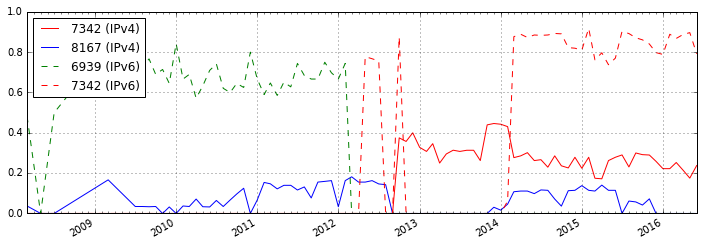
\includegraphics[width=5.0in]{img/j_root_top_upstream.png}
%		\caption{J-Root's most dominant upstream providers}
%		\label{fig:ch04:j_root_top_upstream}
%	\end{subfigure}
%	\begin{subfigure}{1\textwidth}
		\centering
		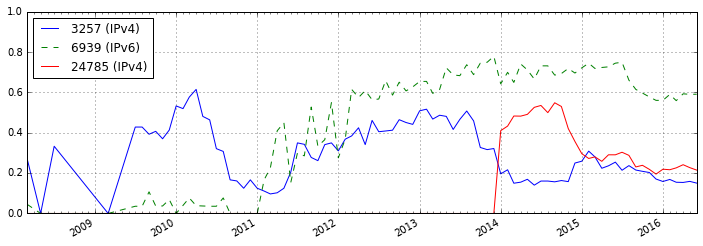
\includegraphics[width=5.0in]{img/m_root_top_upstream.png}
%		\caption{M-Root's most dominant upstream providers}
%		\label{fig:ch04:m_root_top_upstream}
%	\end{subfigure}	
	\caption{M-Root's most dominant upstream providers }
	\label{fig:ch04:top_upstream}
\end{figure}

In contrast to J-Root, M-Root only has five instances where all of them are global nodes and dual-stacked. Low convergence level of M-Root is caused by different routing policies for IPv4 and IPv6 that prefer certain providers to transit. Figure \ref{fig:ch04:top_upstream} illustrates M-Root's top upstream providers as seen by RIS collectors. Since 2011, AS 6939 (Hurricane Electric) has been dominating M-Root's IPv6 upstream (more than 50\%). On the other hand, the IPv4 connectivities are more distributed among several transit providers/peers. The top IPv4 upstream providers are AS 3257 and AS 24785, which are not as dominant as AS 6939 in IPv6. Thus, low convergence level in M-Root case is due to different upstream providers used to reach M-Root.

\subsubsection{Visibility of Root Servers}

As explained in the beginning of this section, Appendix \ref{app:convergence} can also be used to understand the visibility of Root Servers as seen by VPs. %While the nominal is varying for each Root Server, the red line patterns are roughly similar for all, indicating that the number of BGP routers participating in RIS project keeps growing over the time. 
High number of dual-stacked VPs means high level of visibility, or in another word, larger catchment area. The number of VPs are increasing over the time, which is in line with the expansion of the deployed collectors. This is especially noticeable by the end of 2015, where the figure is significantly increased due to the addition of new collectors (Table \ref{table:ch03:ris-collectors}). Ideally, all Root Servers should have relatively similar red line height for a given time, meaning that a similar number of VPs have exposure to those Root Servers. This is not what happens in practice, of course, due to different policies implemented by the operators (amount of deployed instances and its placement, peering agreements, and so on).  
% the nominal of dual-stacked VPs means IPv4 and IPv6 visibility as seen by VPs. The question is, how many VPs that have IPv4 route but not IPv6, and vice versa? don't you think it is more appropriate to represent the visibility?

Large number of instances supposedly should directly correlate to high visibility, while the amount of dual-stacked instances does not have contribution here since the VPs may take any path towards the instances as long as the instances are configured as global nodes. However, this does not always apply. Root Servers with small number of instances (\textless 10)--A, C, and M-Root--have relatively high level of visibility. The lowest ones are F and I-Root, even though both of them have \textasciitilde50 instances. More interestingly, all I-Root instances are configured as global nodes, which should have provided higher exposure to the global Internet. 

We believe that the reason is because F- and I-Root are lacking of peering connection with large providers that are willing to provide global visibility. A- and C-Root are operated by commercial organizations (Verisign and Cogent, respectively) that run large-scale network infrastructures globally. It allows them to provide better connectivities with the rest of the Internet. M-Root peers with a number of of ISPs, with some of them provide free transit service\footnote{\url{http://m.root-servers.org/}}. On the other hand, F- and I-Root use open peering policy that requires participation from the interested organizations. Free peering sessions are typically used to exchange traffic between each others'networks, but not to reach the rest of the Internet. Thus, it limits the visibility of the Root Servers beyond its peers. However, K-Root also implements the same policy but with larger visibility level. We believe that this is due to the status of RIPE as the operator of K-Root, which have large base of membership in its region. Hence, it is easier for RIPE to promote direct peering between K-Root instances and RIPE members.

%In F-Root case, from five of its global nodes, four of them are located in United States, and one is in Amsterdam. 


\subsection{The Trends of AS Path Lengths}
\label{ch04:evolution:as-path-length}
%Dhamdhere et al. \cite{Dhamdhere:2012:MDI:2398776.2398832} concluded that the overall AS path length for IPv6 shows a decreasing trend, and showed sharp decreasing since 2008. As for IPv4, the average AS path length is stable around 4 AS hops.
Appendix \ref{app:path-avg:all-peers} provides the statistics of AS path lengths of VPs toward all selected Root Servers over the observation period. The green line on all graphs illustrates the median of path length, which is summarized in Table \ref{table:ch04:path-length-average}. Except for A and D-Root, Root Servers do not experience much changes on their path lengths over the time. 

Past study shows that the average AS path length tends to get shorter, especially for IPv6  \cite{update}. This is further confirmed by Dhamdhere et al. \cite{Dhamdhere:2012:MDI:2398776.2398832}, who concluded that the overall AS path length for IPv6 shows a decreasing trend, and showed sharp decreasing since 2008. As for IPv4, the average AS path length is stable around 4 AS hops. Result from this thesis indicates roughly similar figure. In general, the average IPv4 and IPv6 path length is marginally less than 4, with the difference between them is not significant. Compared to the rest, K-Root has the shortest path length for both IPv4 and IPv6. It generally shows that K-Root has better reachability as seen by VPs. On the other hand, I-Root have the longest average path length, albeit not that significantly different with the rest. 

Overall, the difference between IPv4 and IPv6 path lengths for each Root Server is not that much. However, convergence level seems to have effect on it. Root Servers with poor convergence level (M- and J-Root) have the highest differences. J-Root have noteworthy lower IPv4 path length compared to its IPv6. On the contrary, M-Root have prominently lower IPv6 path length than its IPv4. It shows that J and M-Root have stronger connectivity on either protocol.

\begin{figure}
	\begin{subfigure}{1\textwidth}
		\centering
		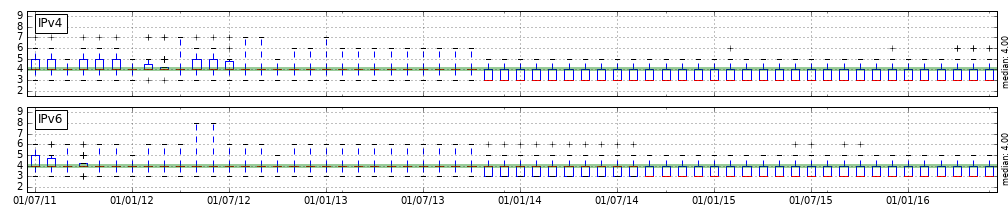
\includegraphics[width=6.5in]{img/path_avg_all_d.png}
		\caption{AS path lengths of D-Root}
		\label{fig:ch04:trends_avg_path_length_d}
	\end{subfigure}
	\begin{subfigure}{1\textwidth}
		\centering
		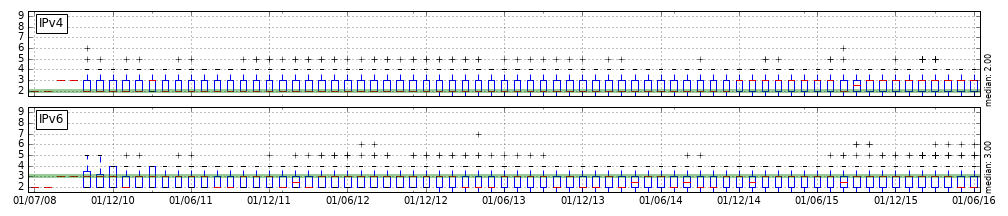
\includegraphics[width=6.5in]{img/path_avg_all_k.png}
		\caption{AS path lengths of K-Root}
		\label{fig:ch04:trends_avg_path_length_k}
	\end{subfigure}
	\begin{subfigure}{1\textwidth}
		\centering
		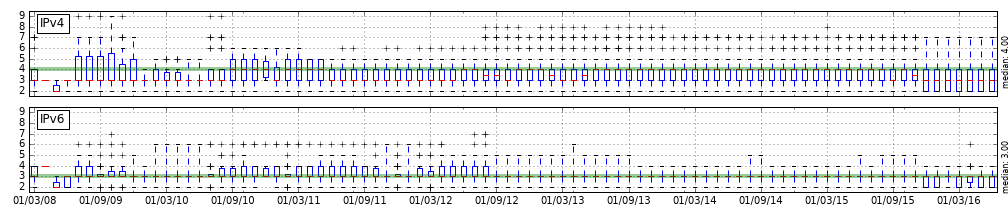
\includegraphics[width=6.5in]{img/path_avg_all_m.png}
		\caption{AS path lengths of M-Root}
		\label{fig:ch04:trends_avg_path_length_m}
	\end{subfigure}
	{\scriptsize \\These are the box plots which represent the distribution of AS path lengths of the respective Root Servers. The central rectangle comprises of three parallel horizontal lines representing the first quartile, the median (red), and the third quartile. The whisker below the rectangle represents the minimum value, while the top whisker is the maximum one. The outlier data is depicted as crosses. The green line represents the average of the median over the time\par}
	\caption{AS path lengths of D, K, and M-Root}
	\label{fig:ch04:trends_avg_path_length}
\end{figure}

%Figure \ref{fig:ch04:trends_avg_path_length} represents selected graphs from Appendix \ref{app:path-avg:all-peers}. D-Root (Figure \ref{fig:ch04:trends_avg_path_length_d}) looks to have two phases of path length dynamism (pre- and post-November 2013), and it will be discussed later. K-Root (Figure \ref{fig:ch04:trends_avg_path_length_k}) 

\begin{table}[!ht]
	\centering
	\begin{tabular}{c c c c c}
		\hline
		\multirow{2}{*}{\textbf{Root Server}} & \multicolumn{2}{c}{\textbf{Median}} & \multicolumn{2}{c}{\textbf{Mean}} \\
		& \textbf{IPv4} & \textbf{IPv6} & \textbf{IPv4} & \textbf{IPv6} \\
		%\textbf{Root Server} & \textbf{IPv4}	& \textbf{IPv6} \\ 
		\hline\hline
		A			& 4 & 3 & 3.79	& 3.64 \\ \hline
		C			& 4 & 4 & 3.68	& 3.77 \\ \hline
		D			& 4 & 4 & 3.78	& 3.75 \\ \hline
		F			& 4 & 4 & 3.65	& 3.67 \\ \hline
		I			& 4 & 4 & 3.86	& 3.90 \\ \hline
		J			& 3 & 3 & 3.18	& 3.62 \\ \hline
		K			& 2 & 3 & 2.56	& 2.65 \\ \hline
		L			& 3 & 3 & 2.95	& 3.03 \\ \hline
		M			& 4 & 3 & 3.68	& 3.10 \\ \hline
	\end{tabular}
	\caption{Median and mean of IPv4 and IPv6 path lengths over the time}
	\label{table:ch04:path-length-average}
\end{table}


Appendix \ref{app:path-avg:all-peers} can be used to see the stability of the AS path length over the time as well.  C, K, and L-Root are relatively stable. It means that there was not major network configuration changes affecting the path length from the VPs. D-Root (Figure \ref{fig:ch04:trends_avg_path_length_d}) looks to have two phases of its path length dynamics. The fluctuated path length of D-Root VPs started to stabilize at November 2013, the same time when D-Root started to use AS 42 as one of their upstream (Section \ref{ch04:evolution:convergence}). This decision seemed to help D-Root gaining lower average path lengths than before, and since then the path length did not vary much. M-Root IPv6 path length (Figure \ref{fig:ch04:trends_avg_path_length_m}) looks similar to D-Root. Starting from September 2012, the path lengths started to stabilize. IPv6 path lengths of M-Root's VPs are mostly 3 (indicated by flat rectangle at 3), which shows that they use an upstream provider that have large connectivities, which is AS 6939 (Figure \ref{fig:ch04:top_upstream}). For A-Root, the path lengths were highly varying until the beginning of 2014, when the length started to stabilize. We believe that the discussion of A-Root in Section \ref{ch04:evolution:convergence} also takes part in this dynamics.

The graphs in Appendix \ref{app:path-avg:all-peers} also inform us about the symmetry of the catchment topology. Ideally, an anycast catchment topology should be in the form of tree(s) where the origin AS of anycast service serves as the center of tree (or their upstream provider(s)), and all end-user ASes should have relatively similar path lengths. It demonstrates that the anycast instances provide good reachability from any corner of the Internet, and that the instances are properly distributed. Quantitatively, this behavior is indicated by a box plot with narrow range of upper and lower whiskers, and as few outliers as possible. C-Root (Figure \ref{fig:path-avg-all-c}) is a good example of it. The extreme contrasting example is M-Root's IPv4 path length. M-Root's poor IPv4 statistics compared to its IPv6 is not because of the overall poor connectivities, but largely contributed by small number of VPs that have quite long paths (marked as outliers in Figure \ref{fig:path-avg-all-m}). It may serve a good indicator on planning new peering agreement or even new instance deployment to provide better connectivities.  



\section{The Differences Between IPv4 and IPv6 Catchment Areas}
\label{ch04:differences}
Previous section discusses about the dynamics of anycast catchment areas over the time in terms of the convergence level and the trends of AS path length. It uses data from all VPs as long as they have both IPv4 and IPv6 routing information toward Root Server. In this section, we focus our discussion on the differences between IPv4 and IPv6 catchment areas itself. Therefore, we focus only on diverging VPs of certain Root Server at a given time. The definition of different AS paths used in this thesis is provided in Section \ref{ch03:analysis}. With current data we have in our disposal, we can not answer the question of \textit{why} exactly the differences take place, since it requires the knowledge of BGP routing configuration on each routers. However, we can find out \textit{to what extent} the differences affecting the catchment areas, as seen from control-plane perspective. 

We start off by discussing the composition of VPs (Section \ref{ch04:diff:composition}). Next, the average path length (Section \ref{ch04:diff:avg-path-length}), followed by how different is it path-length-wise (Section \ref{ch04:diff:diff-how-diff}).

\subsection{Composition of VPs}
\label{ch04:diff:composition}

Different paths encountered by a diverging VP may still result in similar path lengths, or it could also result in either IPv4 or IPv6 shorter path. Section \ref{ch04:evolution:convergence} specifically focuses  on the fraction of converging VPs of all dual-stacked VPs. Here, we are interested to look deeper at the diverging VPs: how many diverging VPs that experience shorter IPv4 path, shorter IPv6 path, or similar path lengths. By breaking down the composition of all VPs based on its IPv4/IPv6 path lengths, we present the results in Appendix \ref{app:peer-composition} with Figure \ref{fig:ch04:composition} showing composition of A and D-Root's VPs serves as an example. Root Servers have more diverging VPs with equal IPv4/IPv6 path lengths than shorter IPv4/IPv6 path, except for J, I, and M-Root. I-Root itself has slightly more diverging VPs with shorter IPv6 paths. Root Servers with low convergence level (J and M-Root) have noticable shorter paths. J-Root is dominated by VPs with shorter IPv4 path. On the contrary, VPs with shorter IPv6 path dominate M-Root.
 

\begin{figure}[!ht]
	\begin{subfigure}{1\textwidth}
		\centering
		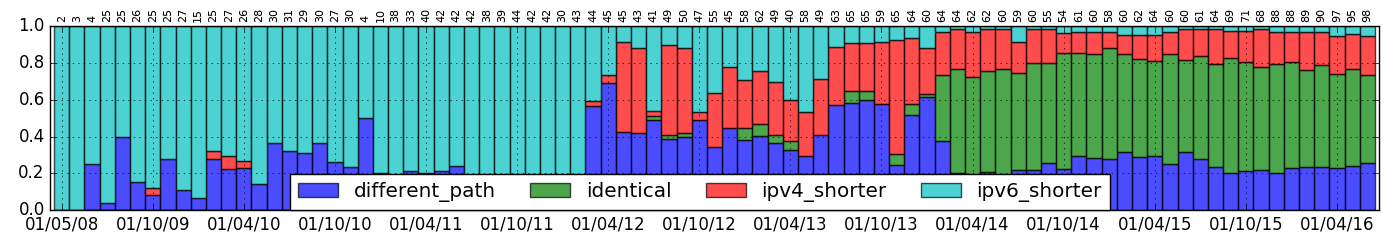
\includegraphics[width=6in]{img/peer_composition_a.png}
		\caption{Composition of A-Root's VPs}
		\label{fig:ch04:composition_a}
	\end{subfigure}
	\begin{subfigure}{1\textwidth}
		\centering
		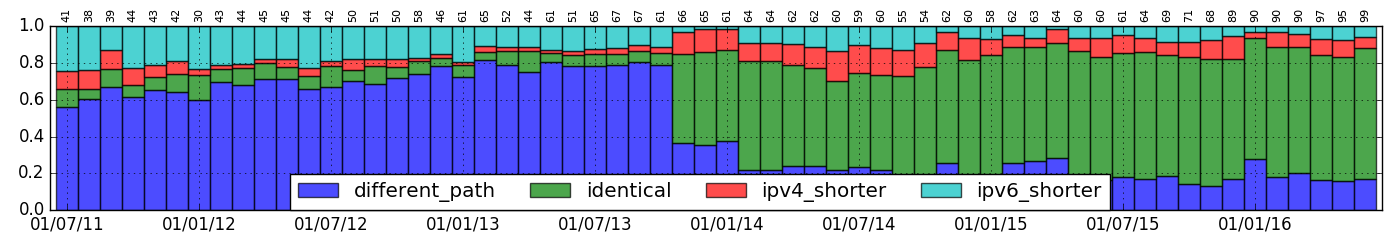
\includegraphics[width=6in]{img/peer_composition_d.png}
		\caption{Composition of D-Root's VPs}
		\label{fig:ch04:composition_d}
	\end{subfigure}	
	{\scriptsize The bins represent the fraction of VPs for each category. The number on top of the bin shows the total number of VPs at a time}
	\caption{Composition of A and D-Root's VPs}
	\label{fig:ch04:composition}
\end{figure}


Diverging paths with equal lengths is largely due to coincidence. However, there are some special cases, for example in D-Root (Figure \ref{fig:ch04:composition_d}). It has large fraction of VPs with diverging path and equal length prior to November 2013. We have discussed in Section \ref{ch04:evolution:convergence} that prior to November 2013, the dominant upstream was AS 22945. AS 22945 itself is identified to have all connectivities by transiting via AS 6939.
The similar case also happens in IPv6, now with AS 10886 as the upstream. In D-Root case, VPs with diverging paths and equal length prior to November 2013 mostly happened because the VPs reached D-Root through AS 22945 for IPv4 and through AS 10886 for IPv6, with AS 6939 as the intermediate transit AS. VPs path via AS 6939 were always the same (regardless IPv4/IPv6), the only difference is the penultimate AS before reaching D-Root's origin AS. After the introduction of AS 42, the catchment topology changed, since most VPs switched to reach D-Root via AS 42.

Prior to February 2012, A-Root (Figure \ref{fig:ch04:composition_a}) was dominated by VPs with shorter IPv6 paths. It is because A-Root directly peered with AS 6939 and all IPv6 connectivities were through them. This is also one of the reasons why A-Root had such low convergence level during that period, as AS 6939 is the dominant IPv6 transit provider thus A-Root's VPs experienced shorter IPv6. Starting in March 2012, they started to use other IPv6 transit providers as well, resulting in the VPs no longer got shorter IPv6. We believe that this event lead to higher A-Root IPv6 path lengths starting from march 2012 in Figure \ref{fig:path-avg-all-a}.

\subsection{Average Path Length}
\label{ch04:diff:avg-path-length}

We have discussed the trends of AS path lengths for all VPs in Section \ref{ch04:evolution:as-path-length}. Here, we focus only on average path length of diverging VPs. The complete result is presented in Appendix \ref{app:path-avg:diff-paths}, and summarized in Table \ref{table:ch04:path-length-average-diff}. To get the knowledge of the quantity of VPs for each AS path lengths, we break down the data to get the VPs degree (relative to the Root Server) in Appendix \ref{app:peer-degree-dist}. 

Intuitively, the longer the path the higher the probability of having diverging paths is. In general, the results in Appendix \ref{app:path-avg:diff-paths} exhibit similar patterns with the ones in Appendix \ref{app:path-avg:all-peers}. This is because of two factors: \textit{(i)} the number of diverging VPs are not significant to influence the overall path length distribution, \textit{(ii)} diverging VPs are generally have longer paths, but not that much, as we see later. Comparing results in Table \ref{table:ch04:path-length-average-diff} and Table \ref{table:ch04:path-length-average}, we see that Root Servers with high convergence level, especially C-, I-, and K-Root, have the largest differences. This is especially noticeable for C-Root, the one with the highest differences (0.53 hop for IPv4 and 0.76 hop for IPv6) by comparing Figure \ref{fig:path-avg-all-c} and Figure \ref{fig:path-avg-diff-c}. The contrast of C-Root's average path lengths between all dual-stacked VPs and diverging VPs only are depicted in Figure \ref{fig:ch04:peer_degree_c}.
Root Servers with low convergence level, J- and M-Root, only slightly differ because the diverging VPs dominate the statistics in Table \ref{table:ch04:path-length-average}. It means that the diverging VPs mostly have longer AS path lengths than the average, thus confirming the hypothesis.

\begin{figure}[!ht]
	\centering
	\begin{subfigure}{1\textwidth}
		\centering
		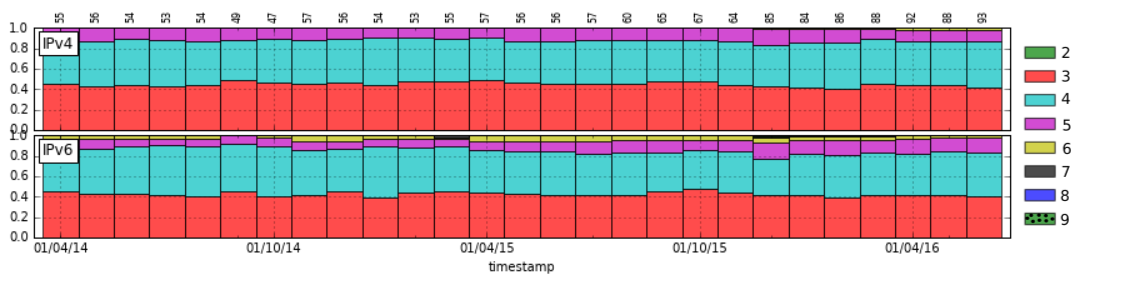
\includegraphics[width=6.5in]{img/peer_degree_all_c.png}
		\caption{All dual-stacked VPs}
		\label{fig:ch04:peer_degree_all_c}
	\end{subfigure}
	\begin{subfigure}{1\textwidth}
	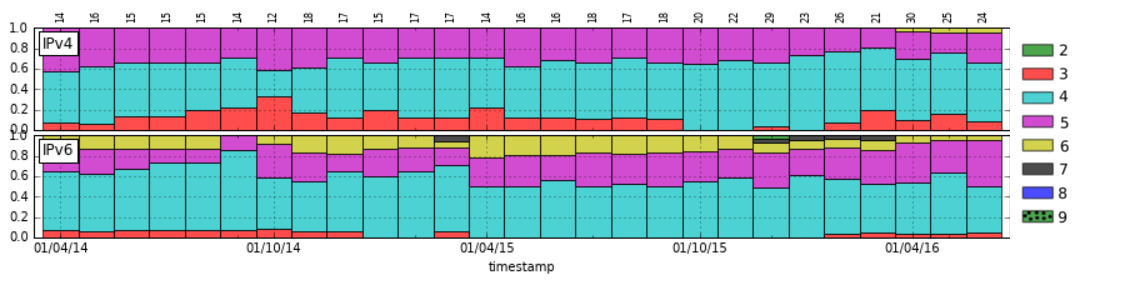
\includegraphics[width=6.5in]{img/peer_degree_diff_c.png}
	\caption{Diverging VPs only}
	\label{fig:ch04:peer_degree_diff_c}
	\end{subfigure}	
	{\scriptsize The bins represent the fraction of VPs for each category. The number on top of the bin shows the total number of VPs at a time}
	\caption{C-Root's VP degree}
	\label{fig:ch04:peer_degree_c}
\end{figure}
 

\begin{table}[!ht]
	\centering
	\begin{tabular}{c c c c c}
		\hline
		%\textbf{Root Server} & \textbf{IPv4}	& \textbf{IPv6} \\ \hline\hline
		\multirow{2}{*}{\textbf{Root Server}} & \multicolumn{2}{c}{\textbf{Median}} & \multicolumn{2}{c}{\textbf{Mean}} \\
		& \textbf{IPv4} & \textbf{IPv6} & \textbf{IPv4} & \textbf{IPv6} \\
		%\textbf{Root Server} & \textbf{IPv4}	& \textbf{IPv6} \\ 
		\hline\hline
		A			& 4 & 4 & 4.03	& 3.82 \\ \hline
		C			& 4 & 4 & 4.21	& 4.53 \\ \hline
		D			& 4 & 4 & 4.09	& 4.04 \\ \hline
		F			& 4 & 4 & 3.83	& 3.88 \\ \hline
		I			& 4 & 4 & 4.29	& 4.37 \\ \hline
		J			& 3 & 4 & 3.20	& 3.70 \\ \hline
		K			& 3 & 3 & 2.86	& 3.13 \\ \hline
		L			& 3 & 3 & 3.09	& 3.24 \\ \hline
		M			& 4 & 3 & 4.00	& 3.22 \\ \hline
	\end{tabular}
	\caption{AS path lengths for diverging VPs}
	\label{table:ch04:path-length-average-diff}
\end{table}

\subsection{How Different Is It?}
\label{ch04:diff:diff-how-diff}
For VPs with either shorter IPv4 or IPv6 paths, it is interesting to find out to what extent the path length difference is. The average differences for shorter IPv4 and IPv6 paths are calculated for each Root Server and presented in Appendix \ref{app:shorter-ipv4} and Appendix \ref{app:shorter-ipv6}, respectively. 

\begin{table}
	\centering
	\begin{tabular}{C{3cm}  C{3cm} C{3cm} }
		\hline
		\textbf{Root Server} & \textbf{Shorter IPv4}	& \textbf{Shorter IPv6}  \\ \hline\hline
		A	& 1.07	& 1.23 \\ \hline
		C	& 1.49	& 1.21 \\ \hline
		D	& 1.12	& 1.09	\\ \hline
		F	& 1.32	& 1.21  \\ \hline
		I	& 1.32	& 1.41 \\ \hline
		J	& 1.41	& 1.16	\\ \hline
		K	& 1.1	& 1.17 \\ \hline
		L	& 1.24	& 1.66	\\ \hline
		M	& 1.03	& 1.43	\\ \hline
	\end{tabular}
	\caption{Average AS path length differences}
	\label{table:ch04:avg_path_diff}
\end{table}

Table \ref{table:ch04:avg_path_diff} summaries the results in Appendix \ref{app:shorter-ipv4} and Appendix \ref{app:shorter-ipv6}. In general, the average AS path difference for both shorter IPv4 and IPv6 is \textasciitilde1 hop. For shorter IPv4 path, C- and J-Root have the largest differences. C-Root (Figure \ref{fig:shorter-ipv4-c}) has consistent number of VPs with 1 and 2 hops of path differences, while J-Root (Figure \ref{fig:shorter-ipv4-j}) used to have varying AS path differences (up to 3 hops) until February 2014. Interestingly, this coincides with the notable increase of its convergence level (Figure \ref{fig:convergence-j}). For shorter IPv6 path, L- and M-Root have the largest differences. Varying path differences (\textgreater1 hop) in L-Root (Figure \ref{fig:app:shorter-ipv6-l}) take place sporadically. However, once it happens, it consists of large differences (3 to 4 hops). For M-Root, the varying path differences started to happen regularly from July 2012.


There is trend among large content providers to conduct direct peerings with networks hosting large number of end-user prefixes, in order to bring their services closer to their clients \cite{Chiu:2015:WOH:2815675.2815719}. This results in one AS hop connection between user and the provider. The similar approach is also indicated to be used by some Root Servers, especially those that implement open peering policy.

One major contributing factor of diverging paths is the practice of direct peering on either IPv4 or IPv6, while the other protocol still need to reach Root Server via transit ASes. Take VP in AS 286 for example. It had diverging paths to reach M-Root between September 1\textsuperscript{st} 2009 to February 1\textsuperscript{st} 2012. AS 286 was directly peered to M-Root for IPv4 connectivity, while for IPv6 it transited via AS 3257. 

Table \ref{table:ch04:direct-peering} presents the fraction of direct peering from VPs with shorter IPv4/IPv6 paths. It should be noted that C- and I-Root origin ASes are run behind their own operators' ASes (Cogent and Netnod, respectively) , hence in their case the direct peering is defined by peering connection between VPs and their upstream ASes. D-Root do not have direct peering because it uses two upstream providers (PCH and MAXGigaPOP) to reach the Internet. For other Root Servers operated by non-profit organizations (F, I, K, L, M), direct peerings between the Root Server's AS and VPs become the major factor of shorter IPv4 path. For shorter IPv6, only K-Root that dominated by direct peering ( 78.4 \%). This shows that IPv6 direct peering is not as common as in IPv4, possibly due to lack of IPv6-enabled ASes to be peered with.

\begin{table}
	\centering
	\begin{tabular}{C{1.5cm}  C{2cm} C{2.5cm} |C{2.5cm} C{2.5cm} }
		\hline
		\textbf{Root Server} & \textbf{Shorter IPv4 (\%)}	& \textbf{Direct peering (\%)} & \textbf{Shorter IPv6 (\%)} & \textbf{Direct peering (\%)} \\ \hline\hline
		A	& 16.86	& 0.98	& 27.3 	& 8.47  \\ \hline
		C	& 8.44	& 38.78 & 2.7 	& 31.91 \\ \hline
		D	& 7.4	& 0 	& 10.46 & 0 	\\ \hline
		F	& 13.08	& 53.65 & 12.42 & 33.78 \\ \hline
		I	& 22.05	& 65.14 & 17.7  & 15.68 \\ \hline
		J	& 42.62	& 34.1 	& 13.66	& 16.78	\\ \hline
		K	& 13.53	& 69.42 & 4.87	& 78.4  \\ \hline
		L	& 12.23	& 51.44 & 4.69	& 27.23	\\ \hline
		M	& 5.95	& 47.48 & 44.84	& 4.12	\\ \hline
	\end{tabular}
	\caption{Fraction of direct peerings from VPs with shorter IPv4 and IPv6}
	\label{table:ch04:direct-peering}
\end{table}

 


%% is there correlation between 

%\subsection{Location of Collectors seeing peers in this category}
%\label{ch04:diff:loc}
%It is interesting to find which RIS collectors that connected to peers with different IPv4/IPv6 paths. While it is true that BGP does not necessarily correlated to physical location \textbf{[citation needed]}, by using this approach we may get a rough understanding about the geographical location of those peers. Appendix \ref{app:physical-loc} presents the result per RIS collector. 

%For Root Servers with low convergence level (Appendix \ref{app:convergence}), namely J and M-Root, their peers with different IPv4/IPv6 paths are frequently detected at all collectors.

%Collector in Sao Paulo has relatively small number of peers detected. However, those peers are frequently detected to have shorter IPv4 path.

%Collector in Frankfurt, RIPE NCC, and Palo Alto have been consistently detecting the most of peers that have IPv4/IPv6 routes to Root Servers. Thus, it is unsurprising to see them frequently detect peers with different IPv4/IPv6 paths (Figure \ref{fig:coll-frankfurt}, \ref{fig:coll-palo-alto}, and \ref{fig:coll-ripe-ncc}). 



%\subsection{Are differences persistent?}
%Sort of small conclusions from previous subsections

\section{Visualizing Anycast Catchment Areas}
\label{ch04:visualizing}
Figure \ref{fig:ch04:vis} represents the result of our tool visualizing J-Root catchment areas as seen by RIS at June 1\textsuperscript{st} 2016. J-Root is selected because it has the lowest convergence level, thus it provides good example for the visualization. Figure \ref{fig:ch04:j-root-6-16} represents the J-Root catchment areas for IPv4 (left) and IPv6 (right) on June 1\textsuperscript{st} 2016. The origin ASes of J-Root prefixes are represented by red star icon. AS level relative to origin ASes is represented by colors: in this example dark blue represents level 1, light blue level 2, orange level 3, and so on. 

From Figure \ref{fig:ch04:j-root-6-16}, it can be immediately seen that J-Root has distinct catchment areas. AS 7342 (marked with yellow circle) was one of the upstream providers used by J-Root. In IPv4 catchment, its role is not significant. Only few VPs reached J-Root through it, possibly due to localization policy. In contrast, AS 7342 becomes the dominant upstream provider in IPv6 catchment, where most of VP paths toward J-Root traversed through it. We may also see that in IPv6 catchment, many VPs has AS 6939 (Hurricane Electric) as their transit AS. This is in contrast with IPv4 catchment where there is no dominant provider as the transit. Thus, this visualization will help operator to get an idea which upstream they use is more dominant than the other. Furthermore, it can be also extended to provide visualization whether their local instance configuration is leaking or not.


\begin{figure}[!ht]
	\begin{subfigure}{1\textwidth}
		\centering
		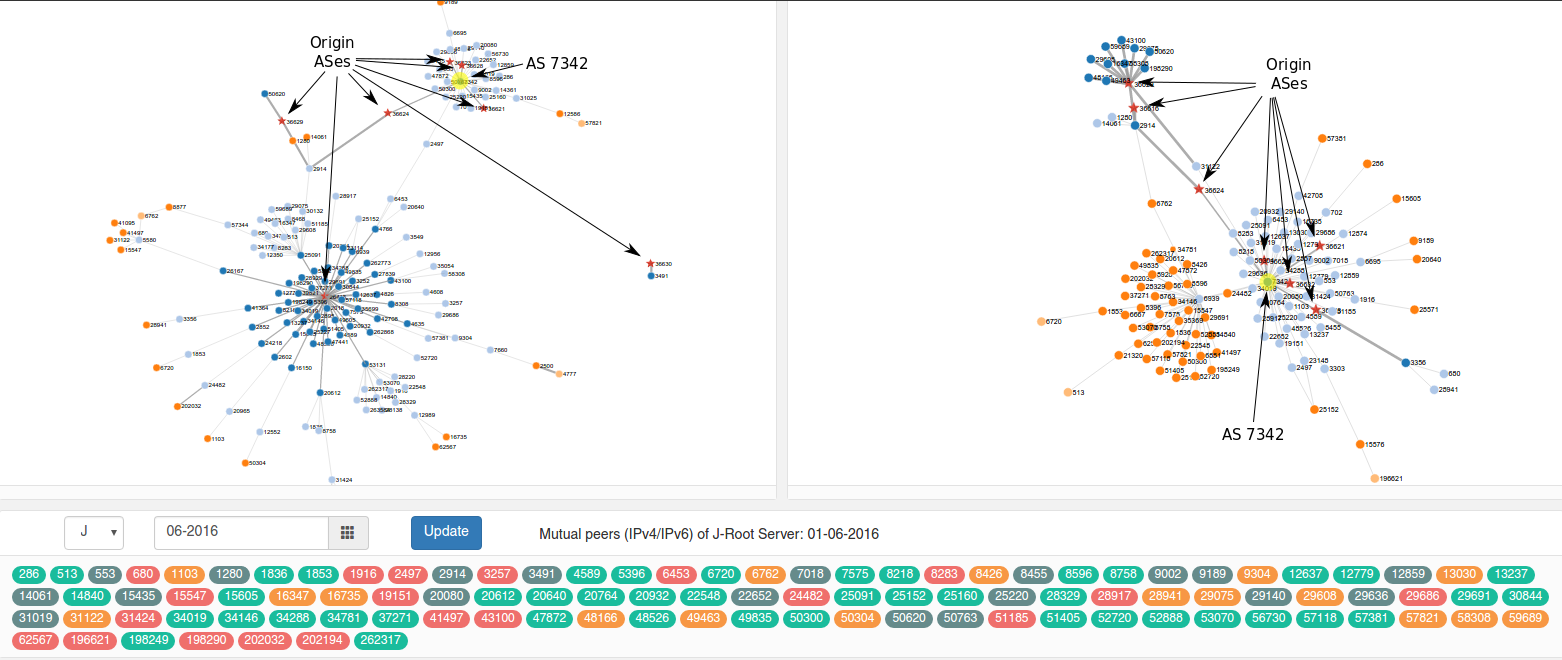
\includegraphics[width=6.5in]{img/j-root-vis}
		\caption{IPv4 (left) and IPv6 (right) catchment areas}
		\label{fig:ch04:j-root-6-16}
	\end{subfigure}
	
	\begin{subfigure}{.5\textwidth}
		\centering
		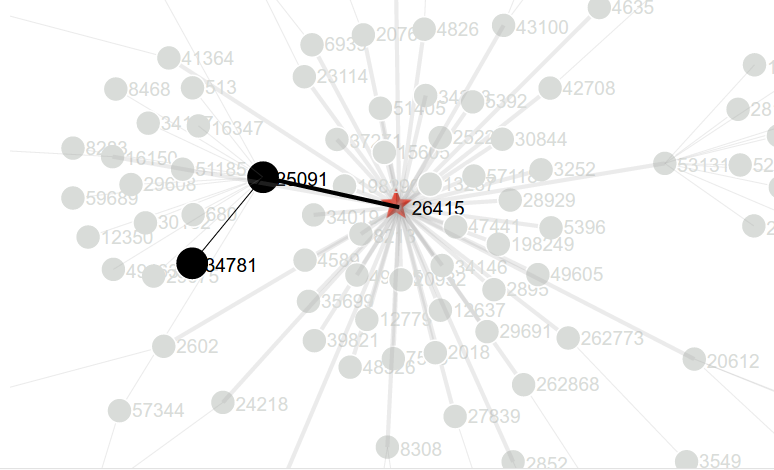
\includegraphics[width=1\linewidth]{img/j-root-as34781-IPv4}
		\caption{IPv4 path for AS 34781}
		\label{fig:ch04:j-root-as34781-4}
	\end{subfigure}	
	\begin{subfigure}{.5\textwidth}
		\centering
		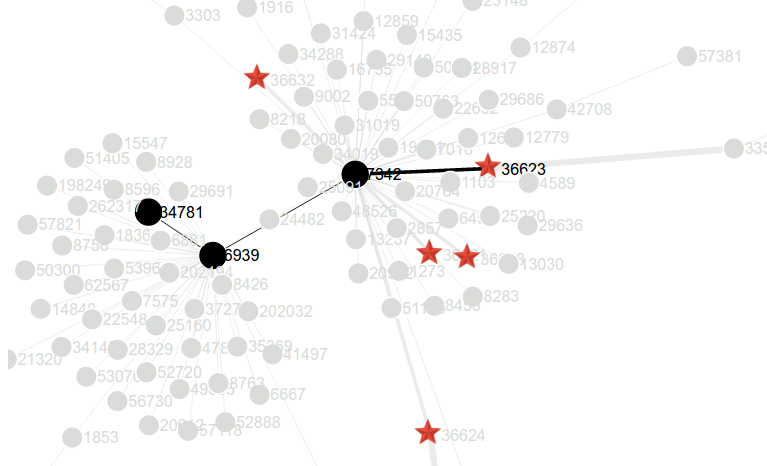
\includegraphics[width=1\linewidth]{img/j-root-as34781-IPv6}
		\caption{IPv6 path for AS 34781}
		\label{fig:ch04:j-root-as34781-6}
	\end{subfigure}	
	\begin{subfigure}{1\textwidth}
		\centering
		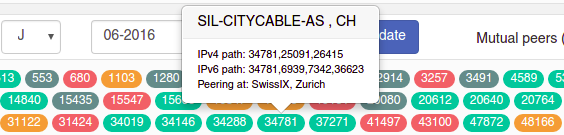
\includegraphics[width=0.8\linewidth]{img/j-root-hover}
		\caption{Hovering to get information about AS information and IPv4/IPv6 paths}
		\label{fig:ch04:j-root-hover}
	\end{subfigure}		
	\caption{Visualization of J-Root catchment areas at June I\textsuperscript{st} 2016}
	\label{fig:ch04:vis}
\end{figure}

\begin{figure}[!ht]
	\centering
	\begin{subfigure}{0.7\textwidth}
		\centering
		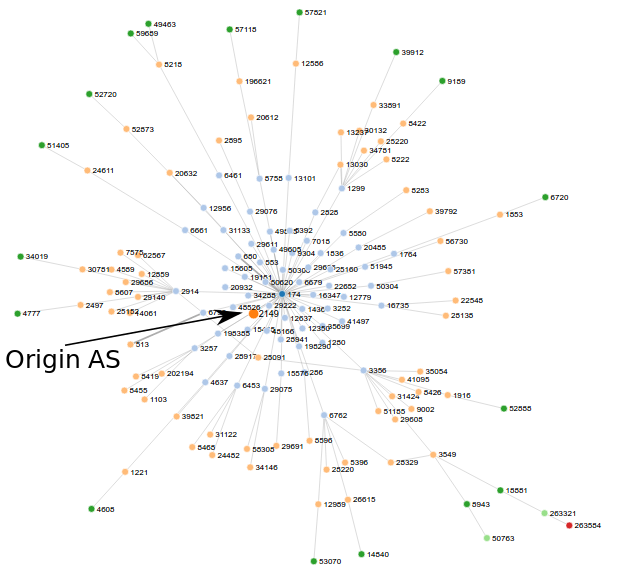
\includegraphics[width=1\linewidth]{img/catchment_c}
		\caption{C-Root}
		\label{fig:ch04:catchment_c}
	\end{subfigure}
	
	\begin{subfigure}{0.7\textwidth}
		\centering
		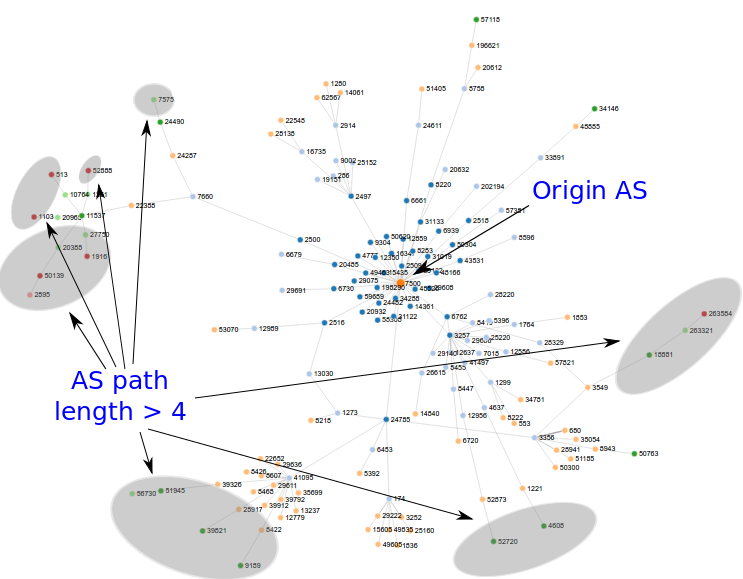
\includegraphics[width=1\linewidth]{img/catchment_m}
		\caption{M-Root}
		\label{fig:ch04:catchment_m}
	\end{subfigure}	
	\caption{C- and M-Root IPv4 catchment areas (January 1\textsuperscript{st} 2016)}
	\label{fig:ch04:catchment}
\end{figure}

On the bottom of Figure \ref{fig:ch04:j-root-6-16}, mutual VPs in both IPv4 and IPv6 catchments are listed. They have different color scheme to represent whether they have identical paths (grey), shorter IPv4 (blue), shorter IPv6 (orange), or diverging path with equal length (red). Hovering one of these mutual VPs will highlight both IPv4 and IPv6 paths, the AS information retrieved from Cymru via \texttt{WHOIS} service, and at which location the VP peers with RIS collector at. Figure \ref{fig:ch04:j-root-hover} shows that AS 34781 is owned by Sil Citycable, a Switzerland-based ISP, and its router is peered with collector at Zurich. The hovering action also results in Figure \ref{fig:ch04:j-root-as34781-4} and \ref{fig:ch04:j-root-as34781-6}. It can be seen that not only it has diverging path, but it also reaches different origin ASes of J-Root (IPv4 uses AS 26415, IPv6 uses AS 36623), which indicates that Sil Citycable customers are served by different J-Root instances for IPv4 and IPv6 queries. 

Recall from Section \ref{ch04:evolution:as-path-length} that an ideal anycast catchment area should be in the form of tree where the origin AS (or its upstream provider's AS) or ASes becomes the center of the tree(s), and the AS path lengths of the end users' ASes should be relatively similar and as short as possible. Poor catchment area would be in the form of a tree where notable number of VPs suffer long AS paths (>4 AS hops\footnote{we base this on the result in \cite{update} which stated that the average AS path length is around 4 AS hops}) and the topology is unbalanced. The presence of notable number of VPs that possess long AS path indicates that the Root Server should provide better connectivity to them. It could be possibly by expanding the direct peering connections or using transit service from ISP with larger footprint in the Internet. If the VPs are identified to be physically far from its closest instance, then it serves as good indicator to add another new instance. 

C-Root is an example of anycasted service of what we believe to have good catchment area (Figure \ref{fig:ch04:catchment_c}), where it has relatively short paths of which enjoyed by all VPs (confirmed in Figure \ref{fig:path-avg-all-c}). On the other hand, IPv4 M-Root (Figure \ref{fig:ch04:catchment_m}) is an example of poor catchment, since there are many VPs suffering from long AS path. This is reflected as well in its average IPv4 path length graph (Figure \ref{fig:path-avg-all-m}) as discussed in Section \ref{ch04:diff:avg-path-length}.

\section{Discussion}
\label{ch04:discussion}
The previous section showed in details about how different IPv4 and IPv6 catchment areas of each Root Servers. Some questions may arise: what does this mean for operator? Does low convergence level automatically mean bad configuration? Above it all, the fundamental question is: \textit{Why assessing the differences is important}? 

As it is already known, IPv6 adoption is still low albeit the accelerating rate \cite{Czyz:2014:MIA:2619239.2626295}. On the other hand, we are now in the phase where IPv6 is already maturing and the major difference between IPv4 and IPv6 is in control-plane \cite{7182788}. This difference itself is expected to get lower, since the IPv6 network deployments are converging to the existing IPv4 networks \cite{Dhamdhere:2012:MDI:2398776.2398832}. While it is true that both networks are in the process of converging, it should be noted however, during the transition period services running on IPv6 should be ensured that they have comparable--if not better--quality as if it is run on IPv4, so that people are encouraged to migrate. It can only be accomplished by understanding the performance of the service on IPv4 and IPv6, and this study--measurement at control-plane level--is one of the necessary efforts. Revealing the differences at control-plane level also means that potential performance problems are revealed as well. As \cite{Dhamdhere:2012:MDI:2398776.2398832} shows, different IPv4 and IPv6 AS paths could lead to much worse performance. This is especially important in anycast, since different routing decision may result in the use of different anycast instances. 

Thus, having good convergence level is preferable for an anycast service, since it more likely provides comparable service quality in both IPv4 and IPv6. However, there is also cases where different path between IPv4 and IPv6 might be useful. For example, if one of the transit AS have congestion that slows down the connection for IPv4 (which cannot detected by BGP), then the IPv6 connection can be used to provide better connectivity.

%People argue that the major factor of slow adoption of IPv6 is due to lack of IPv6 content.

%With the advent of IoT, where devices are connected to the Internet and each of them required its own address, the need to switch to IPv6 becomes eminent.

%C-Root can be considered as a good example. It has quite stable path length (?).


%\section{Concluding Remarks}
%\label{ch04:conclusion}
%Some preliminary conclusion
